\documentclass[tikz,border=3pt]{standalone}
\usepackage{amsmath,amssymb,graphicx}
\usetikzlibrary{arrows.meta,calc,fit,positioning,shapes.geometric}

\begin{document}
\begin{tikzpicture}[
  x=1cm,y=1cm,
  font=\sffamily\scriptsize,
  arr/.style={-{Stealth[length=1.9mm]},draw=black!70,line width=0.55pt},
  softarr/.style={-{Stealth[length=1.7mm]},draw=black!42,line width=0.48pt},
  reuse/.style={draw=black!45,densely dashed,line width=0.5pt},
  bluearr/.style={-{Stealth[length=1.8mm]},draw=blue!55!black,line width=0.65pt},
  box/.style={draw=black!52,rounded corners=1.6pt,fill=white,align=center,inner sep=2.5pt,minimum height=0.67cm},
  scorer/.style={box,draw=teal!65!black,fill=teal!6},
  target/.style={box,draw=orange!78!black,fill=orange!8},
  source/.style={box,draw=violet!65!black,fill=violet!5},
  ref/.style={box,draw=blue!65!black,fill=blue!7},
  prop/.style={box,draw=orange!75!black,fill=orange!9},
  cert/.style={box,draw=red!65!black,fill=red!6},
  final/.style={box,draw=teal!70!black,fill=teal!9,line width=0.8pt},
  neutral/.style={box,draw=black!42,fill=black!2},
  decision/.style={diamond,aspect=1.7,draw=orange!70!black,fill=orange!5,align=center,inner sep=1pt},
  panel/.style={draw=black!32,rounded corners=3pt,line width=0.6pt},
  title/.style={font=\sffamily\small\bfseries,anchor=west},
  note/.style={font=\sffamily\tiny,text=black!60,align=center},
  role/.style={font=\sffamily\scriptsize\bfseries},
]

% ==================================================================
% Panel a: shared frozen scoring substrate
\draw[panel] (0,8.45) rectangle (19,12.35);
\node[title] at (0.20,12.08) {a\quad Frozen Subspace Scoring and Localization};
\node[note,anchor=east] at (18.78,12.10) {illustrative target category $t$: capsule; frozen backbone; support-only fitting};

% Real, auditable capsule assets.
\node[inner sep=0pt] (aqueryimg) at (0.78,10.75)
  {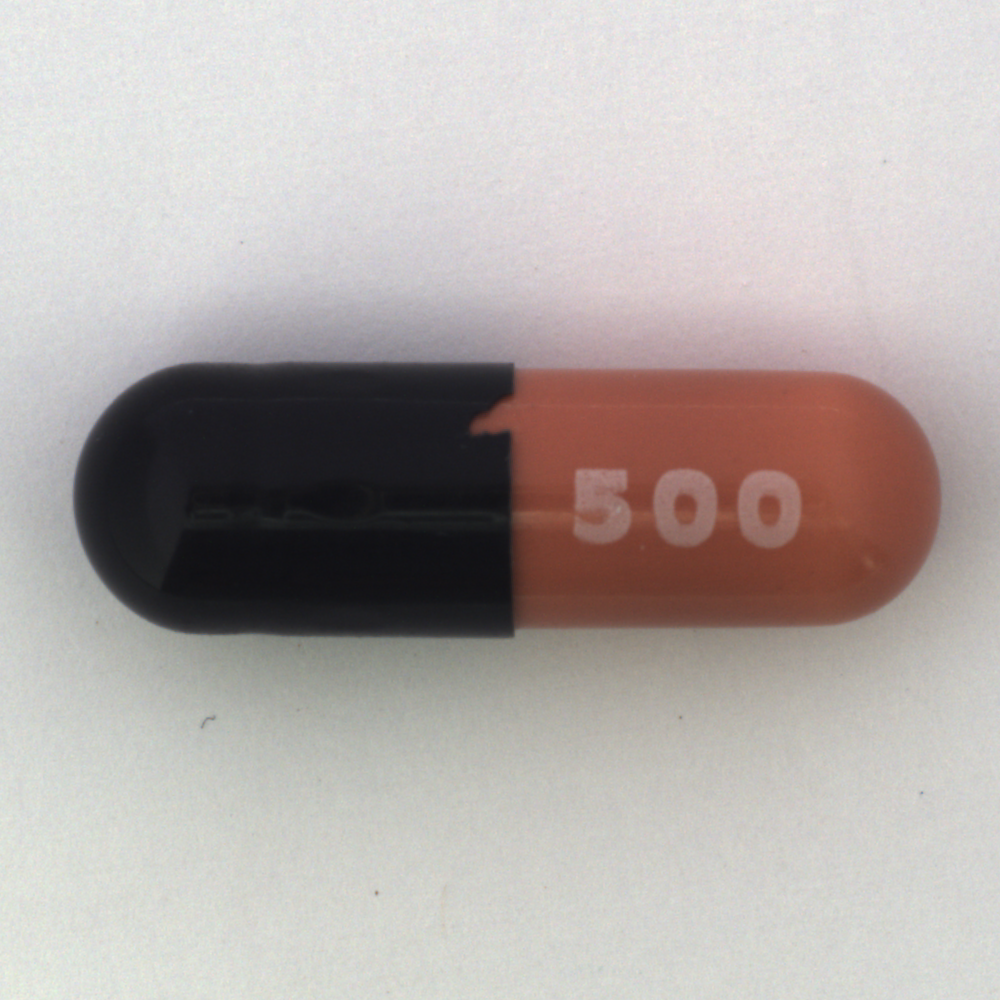
\includegraphics[width=0.72cm]{../../outputs/pipeline_visuals/capsule_k4_seed0/test_capsule_anomaly.png}};
\node[note,anchor=north] at (0.78,10.34) {target query $x_t$};
\node[inner sep=0pt] (asupimg) at (0.92,9.42)
  {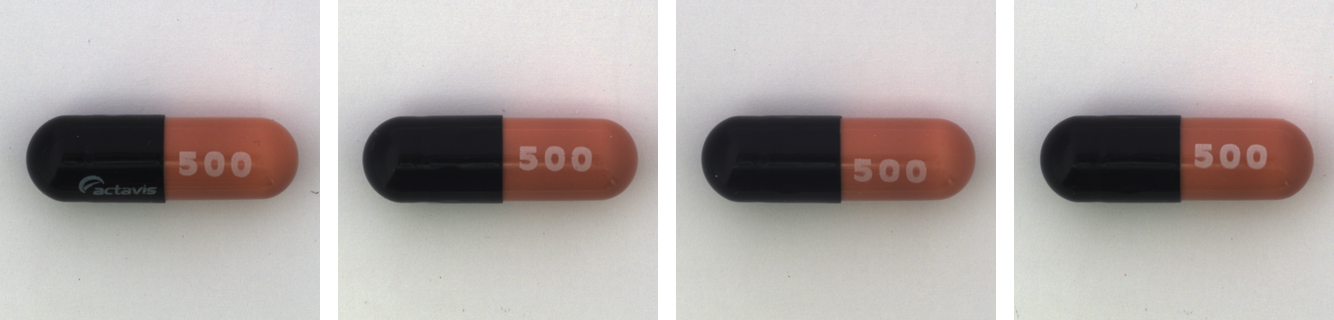
\includegraphics[width=1.55cm]{../../outputs/pipeline_visuals/capsule_k4_seed0/support_montage_k4.png}};
\node[note,anchor=north] at (0.92,9.16) {$k$ target-normal supports $\mathcal S_t$};

\node[ellipse,draw=blue!62!black,fill=blue!6,align=center,minimum width=1.75cm,minimum height=1.22cm] (adino) at (2.75,10.02)
  {frozen DINOv2\\ViT-S/14};

% Compact patch-feature glyphs.
\node[neutral,minimum width=1.45cm] (aqfeat) at (4.65,10.72) {query patch\\features};
\node[neutral,minimum width=1.45cm] (asfeat) at (4.65,9.37) {support patch\\features};

\node[scorer,minimum width=1.70cm,minimum height=1.05cm] (apca) at (6.65,9.38)
  {PCA subspace\\$\mu_t,U_t$};
\node[scorer,minimum width=1.85cm,minimum height=1.05cm] (ares) at (8.85,10.02)
  {orthogonal patch\\residuals $r_t(z)$};
\node[inner sep=0pt] (apatchmap) at (10.65,10.02)
  {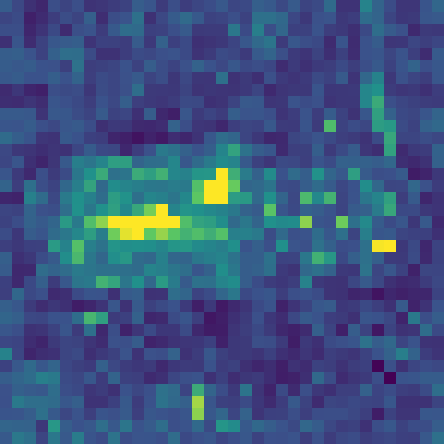
\includegraphics[width=0.92cm]{../../outputs/pipeline_visuals/capsule_k4_seed0/patch_residual_map_nearest.png}};
\node[note,anchor=north] at (10.65,9.50) {patch residual map};
\node[draw=teal!35!black,rounded corners=2pt,fit=(apca)(ares),inner sep=7pt,label={[role]above:PCA residual scorer}] (ascorefit) {};

\node[scorer,minimum width=1.55cm] (aupsample) at (12.55,10.92) {spatial\\upsampling};
\node[inner sep=0pt] (apixelmap) at (14.30,10.92)
  {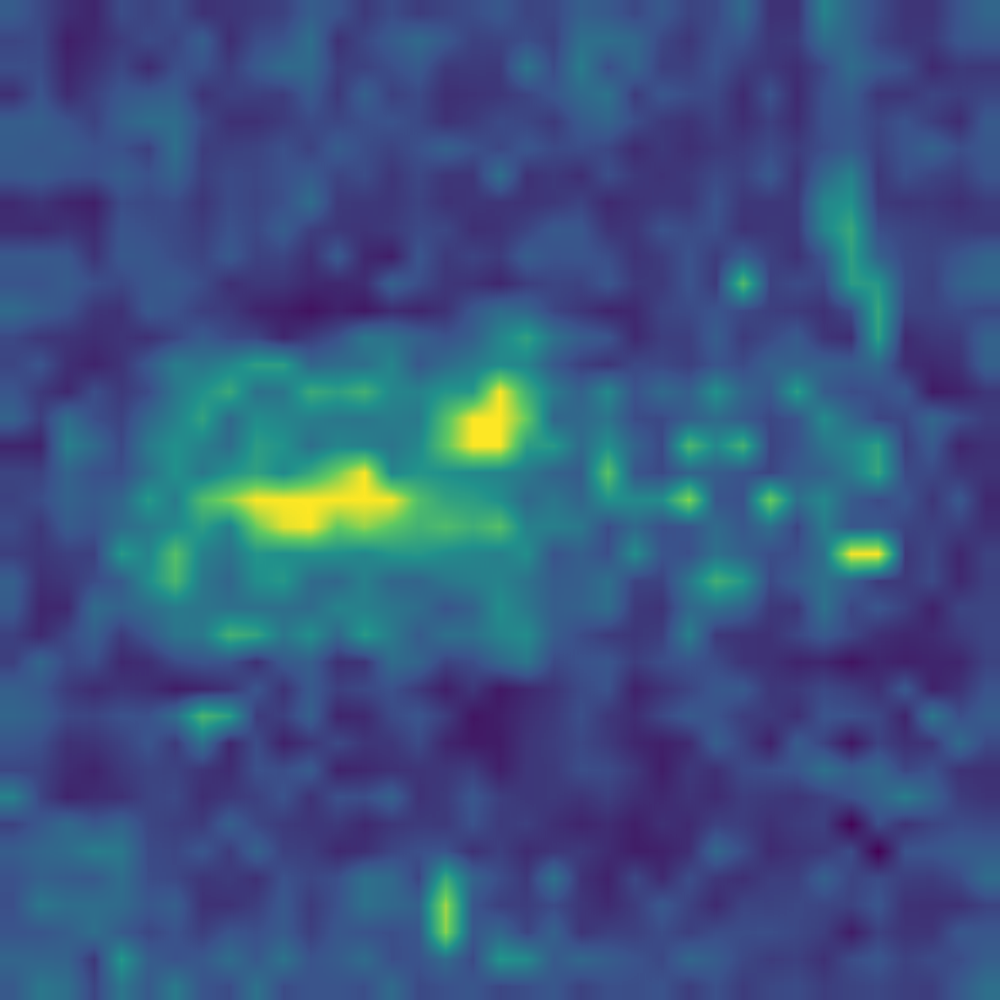
\includegraphics[width=0.92cm]{../../outputs/pipeline_visuals/capsule_k4_seed0/pixel_anomaly_heatmap_bilinear.png}};
\node[note,anchor=north] at (14.30,10.40) {pixel anomaly map};
\node[neutral,minimum width=1.65cm] (apixmetric) at (16.35,10.92) {pixel AUROC\\AU-PRO};

\node[scorer,minimum width=1.72cm] (aaggregate) at (12.55,9.15) {max / top-$\rho$\\aggregation};
\node[final,minimum width=1.60cm] (araw) at (14.55,9.15) {raw score\\$s_t(x)$};
\node[neutral,minimum width=1.65cm] (aimetric) at (16.55,9.15) {image AUROC\\AP};

\draw[arr] (aqueryimg) -- (adino);
\draw[arr] (asupimg) -- (adino);
\draw[arr] (adino) -- (aqfeat);
\draw[arr] (adino) -- (asfeat);
\draw[arr] (asfeat) -- (apca);
\draw[arr] (aqfeat) -- (ares);
\draw[arr] (apca) -- (ares);
\draw[arr] (ares) -- (apatchmap);
\draw[arr] (apatchmap.east) -- ++(0.45,0) |- (aupsample.west);
\draw[arr] (apatchmap.east) -- ++(0.45,0) |- (aaggregate.west);
\draw[arr] (aupsample) -- (apixelmap);
\draw[softarr] (apixelmap) -- (apixmetric);
\draw[arr] (aaggregate) -- (araw);
\draw[softarr] (araw) -- (aimetric);
\node[note,anchor=east] at (18.72,8.67) {evaluation metrics only; neither reliability route changes $s_t(x)$ or the pixel map};

% ==================================================================
% Panel b: target-only route
\draw[panel] (0,5.40) rectangle (19,8.22);
\node[title] at (0.20,7.96) {b\quad Target-Only LOIO Reliability Audit};
\node[note,anchor=east] at (18.78,7.98) {uses only the $k$ target supports; no source categories};

\node[target,minimum width=2.35cm,minimum height=1.05cm] (bloio) at (2.15,6.72)
  {$k$ LOIO scorer fits\\fit on $\mathcal S_t\!\setminus\!\{x_i\}$};
\node[target,minimum width=2.55cm,minimum height=1.05cm] (bcal) at (5.25,6.72)
  {LOIO support calibration\\$\mathcal B_t=\mathcal R_{t,\mathrm{LOIO}}$};
\node[target,minimum width=2.45cm,minimum height=1.05cm] (brank) at (9.15,6.72)
  {target-only rank transform\\$p_{t,\mathrm{LOIO}}(x)$};
\node[decision,minimum width=1.75cm] (bgate) at (12.35,6.72)
  {$p_{t,\mathrm{LOIO}}(x)\leq\alpha$?};
\node[final,minimum width=1.05cm] (balarm) at (14.65,7.18) {alarm};
\node[neutral,minimum width=1.05cm] (bnoalarm) at (14.65,6.25) {no alarm};
\node[note,draw=orange!70!black,fill=orange!8,rounded corners=1.5pt,minimum width=2.65cm,minimum height=0.70cm] (bfloor) at (17.15,6.72)
  {resolution floor\\$p_{\min}=1/(k+1)$};

\draw[arr] (bloio) -- (bcal);
\draw[arr] (bcal) -- (brank);
\draw[arr] (brank) -- (bgate);
\draw[arr,draw=teal!65!black] (bgate.north east) |- (balarm.west);
\draw[arr,draw=red!70!black] (bgate.south east) |- (bnoalarm.west);
\draw[arr] (araw.south) -- ++(0,-0.34) -| node[note,pos=0.70,right] {full-support score $s_t(x)$} (brank.north);

% ==================================================================
% Panel c: source-side CRESS and conditional target use
\draw[panel] (0,0) rectangle (19,5.18);
\node[title] at (0.20,4.92) {c\quad CRESS Source-Side Threshold Certification};
\node[note,anchor=east] at (18.78,4.94) {known-normal source archives only; target test data and labels never enter selection};

% Non-target source-category pool (each category owns both inputs below).
\node[source,text width=2.05cm,minimum height=1.05cm] (csourcepool) at (1.25,3.25)
  {non-target source categories\\grid $\cdot$ leather $\cdot$ hazelnut\\metal nut $\cdot\,\ldots$};
\node[note,anchor=north] at (1.25,2.58) {for every category $c\ne t$};

% Two inputs for every source category.
\node[source,text width=1.35cm] (csupport) at (3.45,4.00) {$k$ source supports\\$\mathcal S_c$};
\node[source,text width=1.45cm] (carchive) at (3.45,2.35) {held-out good archive\\$\mathcal A_c^{\mathrm{src}}$};

\node[target,text width=1.45cm] (cloiocal) at (5.30,4.00)
  {LOIO calibration\\$\mathcal B_c$};
\node[note,anchor=north] at (5.30,3.57) {same construction as (b)};
\node[target,text width=1.35cm] (cstats) at (7.15,4.00)
  {support statistics\\$m_c,d_c$};

\node[note,draw=black!38,rounded corners=1.4pt,fill=black!2,text width=1.35cm,minimum height=0.75cm] (cviews) at (5.25,2.25)
  {fixed audit views\\clean / shifted};
\node[scorer,text width=1.45cm,minimum height=0.92cm] (cscorer) at (7.15,2.25)
  {scorer from (a)\\category-specific fit};
\node[source,text width=1.35cm] (craw) at (9.00,2.25)
  {raw score views\\$s_c(x^{(d)})$};

\node[source,text width=1.35cm,minimum height=0.92cm] (cnorm) at (9.00,3.82)
  {support-only\\normalization};
\node[source,text width=1.25cm,minimum height=0.90cm] (cselect) at (10.72,3.82)
  {select /\\aggregate views};
\node[note,anchor=north] at (10.72,3.25) {matched / clean / agnostic / control};
\node[neutral,text width=1.10cm,minimum height=0.92cm] (csplit) at (12.30,3.82)
  {disjoint\\category split};

\node[ref,text width=1.00cm] (cref) at (13.75,4.38) {$\mathcal R$\\Reference};
\node[prop,text width=1.00cm] (cprop) at (13.75,3.28) {$\mathcal P$\\Proposal};
\node[cert,text width=1.00cm] (ccert) at (13.75,2.18) {$\mathcal C$\\Certification};

\node[ref,text width=1.45cm] (crefmap) at (15.45,4.38)
  {reference map\\$p_{\mathcal R}(\cdot)$};
\node[prop,text width=1.55cm] (candidates) at (15.45,3.28)
  {proposal p-values\\candidates $\mathcal T$};
\node[cert,text width=1.55cm] (closs) at (15.45,2.18)
  {category losses\\$L_c(\tau),\bar L_{\mathcal C}(\tau)$};

\node[cert,text width=1.70cm] (cucb) at (15.05,1.05)
  {Hoeffding category-risk\\UCB $U_{\mathrm H}(\tau)$};
\node[final,text width=2.70cm,minimum height=1.02cm] (ctau) at (17.45,1.10)
  {passing set and fallback\\$\mathcal T_{\rm pass}=\{\tau:U_{\mathrm H}(\tau)\leq\alpha\}$\\$\tau^\star=\max(\mathcal T_{\rm pass}\cup\{0\})$};

% Source-score construction.
\draw[arr] (csourcepool.east) -- ++(0.20,0) |- (csupport.west);
\draw[arr] (csourcepool.east) -- ++(0.20,0) |- (carchive.west);
\draw[arr] (csupport) -- (cloiocal);
\draw[arr] (cloiocal) -- (cstats);
\draw[arr] (carchive) -- (cviews);
\draw[arr] (cviews) -- (cscorer);
\draw[arr] (csupport.south) -- ++(0,-0.35) -| node[note,pos=0.78,above] {full-support fit} (cscorer.north);
\draw[arr] (cscorer) -- (craw);
\draw[arr] (cstats) -- (cnorm);
\draw[arr] (craw) -- (cnorm);
\draw[arr] (cnorm) -- (cselect);
\draw[arr] (cselect) -- (csplit);
\draw[arr] (csplit.east) -- ++(0.18,0) |- (cref.west);
\draw[arr] (csplit.east) -- (cprop.west);
\draw[arr] (csplit.east) -- ++(0.18,0) |- (ccert.west);

% R/P/C statistical roles.
\draw[arr] (cref) -- (crefmap);
\draw[arr] (cprop) -- (candidates);
\draw[arr] (ccert) -- (closs);
\draw[bluearr] (crefmap.south) -- (candidates.north);
\draw[bluearr] (crefmap.east) -- ++(0.30,0) |- (closs.east);
\draw[arr] (candidates.south) -- (closs.north);
\draw[arr] (closs.south) -- (cucb.north);
\draw[arr] (cucb) -- (ctau);

% Reuse annotation, explicitly not a shared-data arrow.
% Conditional deployment strip: explains relevance to the target without overclaiming.
\node[note,draw=blue!40!black,densely dashed,rounded corners=1.3pt,fill=blue!2,
      minimum width=9.1cm,minimum height=0.48cm] at (9.45,0.38)
  {conditional target use: $\widetilde s_t(x)\xrightarrow{\ p_{\mathcal R}(\cdot)\ }p_{\mathcal R}(x)\leq\tau^\star$;
   target control additionally requires source-risk dominance or category exchangeability};

\end{tikzpicture}
\end{document}
